\documentclass[11pt,a4paper]{article}

\usepackage[T1]{fontenc}
\usepackage[utf8]{inputenc}
\usepackage{lmodern}
\usepackage[english]{babel}
\usepackage[margin=2.3cm]{geometry}
\usepackage{graphicx}
\usepackage{booktabs}
\usepackage{array}
\usepackage{xcolor}
\usepackage{caption}
\usepackage{float}
\usepackage{enumitem}
\usepackage[hidelinks]{hyperref}

\definecolor{primary}{HTML}{1F3B6E}
\definecolor{accent}{HTML}{E26D3C}
\captionsetup{font=small,labelfont={bf,color=primary}}
\graphicspath{{../results/figures/}{../results/confusion_matrices/}}
\setlength{\parskip}{0.5em}
\setlength{\parindent}{0pt}
\renewcommand{\arraystretch}{1.15}

\newcommand{\sectionrule}{\textcolor{accent}{\rule{\linewidth}{1.2pt}}}

\begin{document}

% ----------------------------- Title page ------------------------------
\begin{titlepage}
\centering
\vspace*{2.2cm}
{\color{primary}\Huge\bfseries Predicting User Sentiment\\[0.3cm] in Software Issue Reports\par}
\vspace{0.6cm}
\sectionrule\par
\vspace{0.6cm}
{\Large A machine learning pipeline that classifies application reviews as\\
negative, neutral or positive\par}
\vspace{2.2cm}
{\large\bfseries Yann MASSOUAM \quad$\cdot$\quad Vénus BAKIKO \quad$\cdot$\quad Faïçal DIELO\par}
\vspace{0.8cm}
{\large ST2MLE : Machine Learning for IT Engineers\par}
\vspace{0.4cm}
{\large Project report\par}
\vfill
{\small All figures and numbers in this report are produced by \texttt{python main.py}
and are fully reproducible (global seed \texttt{RANDOM\_STATE = 42}).\par}
\end{titlepage}

% ----------------------------- 1. Overview -----------------------------
\section{Project overview}
This project builds and evaluates a complete machine learning pipeline that reads
the text of an application review and predicts its sentiment among three classes:
negative, neutral and positive. The task is a supervised, multi class text
classification problem. Our goal is not only to obtain a working classifier, but
also to compare several ways of turning text into numbers and several classification
algorithms, and to justify every design choice with measured evidence.

The study compares four vectorisation strategies (Bag of Words, TF\,IDF, a Word2Vec
model trained on our own corpus, and the pre trained Word2Vec vectors from Google
News) against five classifiers (Naive Bayes, Decision Tree, Random Forest, AdaBoost
and Logistic Regression). Each classifier is tuned with five fold cross validation.
Four dedicated experiments then study class imbalance handling, dimensionality
reduction, decision tree pruning and early stopping.

% ----------------------------- 2. Dataset ------------------------------
\section{Dataset}
\subsection{Source and labels}
We use a real, pre cleaned dataset of Facebook application reviews downloaded from
Kaggle. Each row contains the review text and a star rating from one to five. We turn
the rating into a sentiment label with the usual convention: one or two stars become
negative, three stars become neutral, and four or five stars become positive. This
choice is convenient and standard, but it is worth keeping in mind that a star rating
is only a proxy for sentiment, which is one reason the neutral class is genuinely
hard.

\subsection{Composition}
The same short review (for example ``good'' or ``nice'') appears thousands of times,
so we remove duplicate texts. This matters for a subtle but important reason: if an
identical text appeared in both the training and the test set, the model would be
evaluated on something it had already seen, and the score would be optimistic. After
de duplication and after dropping reviews that become empty once cleaned, 5\,923
unique reviews remain. The class distribution is strongly imbalanced, which is itself
realistic for app stores where most reviews are positive.

\begin{table}[H]
\centering
\begin{tabular}{lccc}
\toprule
\textbf{Class} & \textbf{From rating} & \textbf{Count} & \textbf{Share} \\
\midrule
positive & 4 to 5 stars & 3\,801 & 64.2\,\% \\
negative & 1 to 2 stars & 1\,857 & 31.4\,\% \\
neutral  & 3 stars      & 265    & 4.5\,\% \\
\bottomrule
\end{tabular}
\caption{Class distribution after cleaning and de duplication. Positives outnumber
neutrals by roughly fourteen to one.}
\end{table}

\begin{figure}[H]
\centering
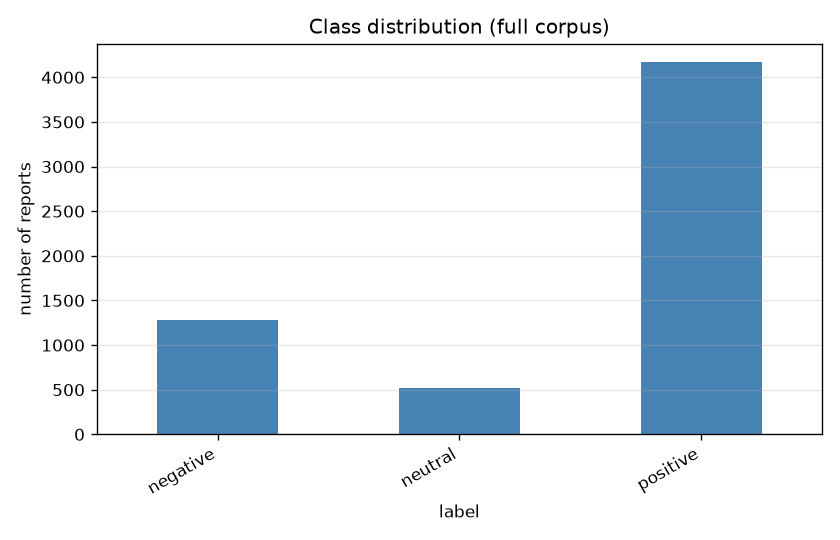
\includegraphics[width=0.62\linewidth]{class_distribution.png}
\caption{Number of reviews per class. The neutral class is tiny, which drives most of
the difficulty discussed later.}
\end{figure}

% ----------------------------- 3. Pipeline -----------------------------
\section{The pipeline, step by step}
The pipeline reads from left to right as follows: raw text, preprocessing,
vectorisation, optional balancing, optional dimensionality reduction, a tuned
classifier, and finally evaluation. Two engineering decisions keep the whole study
both fast and correct. First, preprocessing learns nothing from the data, so it runs
a single time up front rather than inside every cross validation fold. Second, the
fitted vectorisers are cached, so the expensive Word2Vec and TF\,IDF computations are
reused across every hyper parameter combination. As a result the complete study runs
in roughly eight minutes on four cores.

\subsection{Preprocessing}
We lower case the text, remove URLs, punctuation and digits, tokenise, remove common
stop words, and lemmatise. Two choices deserve a comment. We deliberately keep
negation words such as ``not'', ``no'' and ``never'', because they flip the sentiment
and removing them as ordinary stop words would destroy useful signal. We also apply a
light two pass lemmatisation that maps ``crashing'' to ``crash'' and ``issues'' to
``issue'', which shrinks the vocabulary without the cost of a full grammatical
analyser. As an example, ``Critical issue, the app keeps crashing'' becomes ``critical
issue app keep crash''.

\subsection{Vectorisation}
Models only understand numbers, so each review is turned into a vector. We compare the
four representations named in the brief.

\begin{table}[H]
\centering
\begin{tabular}{lll}
\toprule
\textbf{Method} & \textbf{Idea} & \textbf{Output} \\
\midrule
Bag of Words & counts how often each word appears & sparse, non negative \\
TF\,IDF & counts re weighted by how rare a word is & sparse, non negative \\
Word2Vec & mean of embeddings trained on our reviews & dense \\
Word2Vec pre trained & mean of Google News 300d vectors & dense \\
\bottomrule
\end{tabular}
\caption{The four vectorisers. Sparse and non negative outputs feed Multinomial Naive
Bayes; dense outputs use the Gaussian variant, selected automatically.}
\end{table}

Keeping both an in domain Word2Vec and the pre trained Google News Word2Vec lets us
contrast learning embeddings on our own data against reusing embeddings learned on a
very large external corpus. A BERT vectoriser is also implemented and documented; it
needs the model hub, which is not reachable in our environment, so it is skipped
automatically and provided through a script that runs wherever the hub is available.

\subsection{Classifiers}
We compare five classifiers. Naive Bayes estimates word probabilities per class and
assumes the words are independent; this assumption is false in practice but works
very well and is fast in high dimension. The Decision Tree is interpretable but tends
to over fit, which motivates pruning. The Random Forest averages many decorrelated
trees. AdaBoost combines very shallow trees and focuses on hard cases. Logistic
Regression draws a regularised linear boundary and serves as a robust baseline. Naive
Bayes is chosen automatically as the multinomial variant for sparse counts and the
Gaussian variant for dense embeddings, so that its assumptions match the data.

% ----------------------------- 4. Methodology --------------------------
\section{Experimental methodology}
We split the data into 80\,\% training and 20\,\% test, in a stratified way so that
the class proportions are preserved in both parts. On the training set we run five
fold stratified cross validation, and we tune every classifier with a grid search
that maximises the macro averaged F1 score. The test set is touched only once, at the
very end, to report the final numbers. Every stochastic component is seeded, so a
clean run reproduces the same results.

% ----------------------------- 5. Metrics ------------------------------
\section{Understanding the metrics in this context}
Because the classes are computed one against the rest, each metric is defined per
class and then averaged. For a given class, a true positive is a review that truly
belongs to the class and is predicted as such, a false positive is predicted as the
class but does not belong to it, and a false negative is a true member of the class
that the model missed.

\begin{itemize}[leftmargin=1.4em]
\item \textbf{Accuracy} is the share of correctly classified reviews. On an
imbalanced problem it is misleading, because a model can score high simply by always
predicting the dominant class.
\item \textbf{Precision} of a class answers the question: when the model predicts this
class, how often is it right. It measures the reliability of the alerts.
\item \textbf{Recall} of a class answers: among the reviews that truly belong to this
class, how many does the model recover. It measures coverage.
\item \textbf{F1} is the harmonic mean of precision and recall, so it is low whenever
either of the two is low.
\item \textbf{Macro F1} is the simple average of the three per class F1 scores. It
treats every class equally, so neglecting the rare class is heavily penalised.
\end{itemize}

This is exactly why we tune on the macro F1 rather than on the accuracy. On a corpus
that is 64\,\% positive, the accuracy rewards a model that ignores the minority
classes, whereas the macro F1 and the per class recall expose that behaviour
immediately.

% ----------------------------- 6. Results ------------------------------
\section{Results: model comparison}
The table below reports the test set results for all twenty combinations, sorted by
macro F1. The accompanying chart shows the same information visually.

\begin{table}[H]
\centering
\small
\begin{tabular}{rllccccc}
\toprule
\# & \textbf{Vectoriser} & \textbf{Classifier} & \textbf{CV F1} & \textbf{Acc.} & \textbf{Prec.} & \textbf{Rec.} & \textbf{F1 macro} \\
\midrule
1  & TF\,IDF & Naive Bayes & 0.550 & 0.839 & 0.550 & 0.569 & \textbf{0.559} \\
2  & TF\,IDF & Logistic Regression & 0.557 & 0.830 & 0.547 & 0.563 & 0.555 \\
3  & TF\,IDF & Random Forest & 0.541 & 0.824 & 0.540 & 0.558 & 0.548 \\
4  & BoW & Naive Bayes & 0.569 & 0.817 & 0.542 & 0.554 & 0.548 \\
5  & BoW & Logistic Regression & 0.561 & 0.806 & 0.550 & 0.545 & 0.546 \\
6  & Word2Vec pre trained & Random Forest & 0.535 & 0.821 & 0.542 & 0.545 & 0.542 \\
7  & BoW & Decision Tree & 0.533 & 0.768 & 0.547 & 0.533 & 0.539 \\
8  & BoW & Random Forest & 0.542 & 0.810 & 0.534 & 0.542 & 0.537 \\
9  & Word2Vec & Logistic Regression & 0.532 & 0.810 & 0.527 & 0.547 & 0.537 \\
10 & Word2Vec pre trained & Logistic Regression & 0.558 & 0.802 & 0.525 & 0.544 & 0.535 \\
11 & Word2Vec & Random Forest & 0.539 & 0.801 & 0.520 & 0.542 & 0.530 \\
12 & TF\,IDF & Decision Tree & 0.527 & 0.784 & 0.578 & 0.530 & 0.528 \\
13 & Word2Vec & Naive Bayes & 0.517 & 0.685 & 0.542 & 0.537 & 0.518 \\
14 & Word2Vec & AdaBoost & 0.518 & 0.780 & 0.503 & 0.531 & 0.516 \\
15 & Word2Vec pre trained & AdaBoost & 0.527 & 0.783 & 0.506 & 0.527 & 0.516 \\
16 & Word2Vec & Decision Tree & 0.533 & 0.763 & 0.496 & 0.514 & 0.505 \\
17 & Word2Vec pre trained & Decision Tree & 0.506 & 0.746 & 0.483 & 0.504 & 0.493 \\
18 & TF\,IDF & AdaBoost & 0.459 & 0.757 & 0.512 & 0.471 & 0.472 \\
19 & BoW & AdaBoost & 0.454 & 0.753 & 0.516 & 0.463 & 0.465 \\
20 & Word2Vec pre trained & Naive Bayes & 0.444 & 0.630 & 0.465 & 0.479 & 0.455 \\
\bottomrule
\end{tabular}
\caption{Full comparison on the held out test set, sorted by macro F1.}
\end{table}

\begin{figure}[H]
\centering
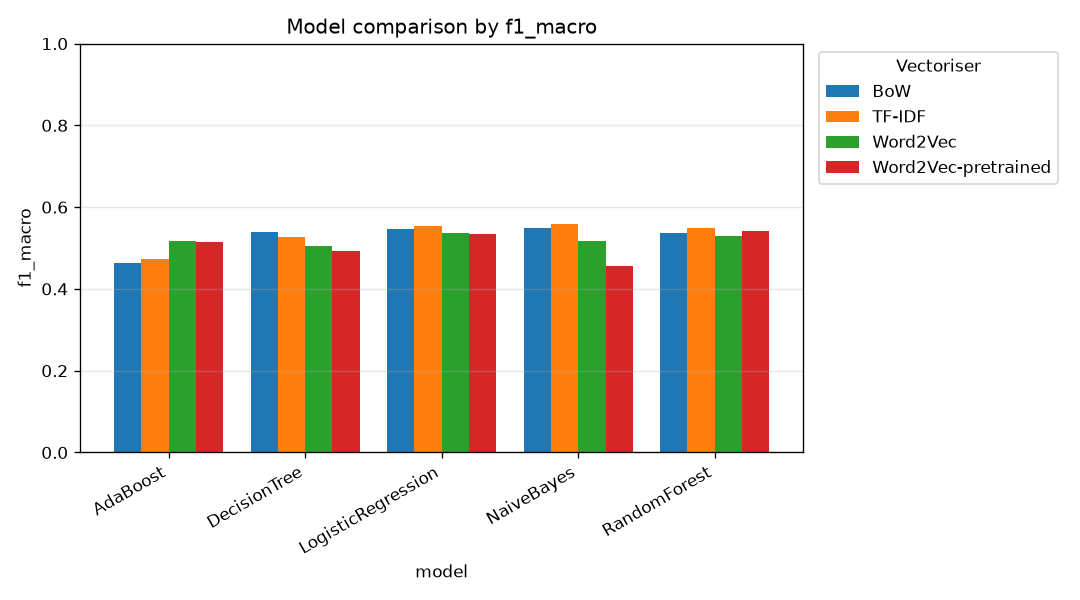
\includegraphics[width=0.85\linewidth]{comparison_f1.png}
\caption{Macro F1 of every classifier grouped by vectoriser.}
\end{figure}

Several lessons stand out. The best combination is TF\,IDF with Naive Bayes at 0.559
macro F1, and the five best entries are all sparse count methods. On short and noisy
review text, counting the right words and weighting them by rarity beats averaging
dense embeddings, because the mean of word vectors tends to wash out the few strong
sentiment words that a short review relies on. AdaBoost sits at the very bottom,
because its shallow stumps can only test one word at a time out of several thousand.
The pre trained Word2Vec behaves reasonably with the Random Forest, where it reaches
0.542 and ranks sixth, but it is the worst entry with Gaussian Naive Bayes at 0.455.
This is a useful reminder that a pre trained representation is not automatically
better than one learned on the data at hand, and that the classifier has to match the
geometry of the features. Finally, the scores cluster tightly between 0.46 and 0.56,
which is the honest signature of a real and difficult problem rather than a sign that
the models are interchangeable.

\section{The trap of accuracy}
The best model deserves a closer look, because its confusion matrix tells a story
that the accuracy hides.

\begin{figure}[H]
\centering
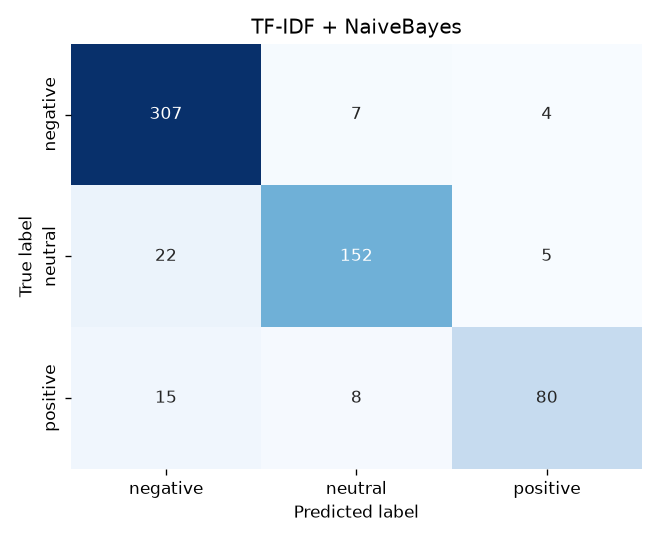
\includegraphics[width=0.5\linewidth]{TF-IDF_NaiveBayes.png}
\caption{Confusion matrix of the best model (TF\,IDF with Naive Bayes) on the test
set. Rows are the true class, columns the predicted class.}
\end{figure}

Reading the matrix, the entire neutral column is empty. In other words, the model
never predicts the neutral class even once. The 53 truly neutral reviews are all sent
to either negative or positive. The consequence is striking. The accuracy is 0.839,
which looks excellent, and the weighted F1 reaches 0.819, yet the macro F1 is only
0.559 because the neutral F1 is exactly zero. The per class numbers confirm this: the
negative class reaches a precision of 0.786 and a recall of 0.782, the positive class
reaches a precision of 0.863 and a recall of 0.925, while the neutral class scores
zero on every metric. The lesson is methodological and central to our work: on an
imbalanced dataset the accuracy can be very high while an entire class is ignored, so
the macro F1 and the per class recall are the numbers that actually matter.

% ----------------------------- 7. Imbalance ----------------------------
\section{Handling class imbalance}
To address the imbalance we compare three strategies on a fixed pipeline that uses
TF\,IDF features and a Logistic Regression. Only the resampling step changes, and it
is applied inside the pipeline so that it acts on the training folds alone and never
on the test data.

\begin{table}[H]
\centering
\begin{tabular}{lcccc}
\toprule
\textbf{Strategy} & \textbf{Accuracy} & \textbf{Macro F1} & \textbf{Recall neg.} & \textbf{Recall neu.} \\
\midrule
none (baseline) & 0.836 & 0.555 & 0.745 & 0.000 \\
SMOTE & 0.727 & 0.551 & 0.758 & 0.189 \\
under sampling & 0.601 & 0.505 & 0.637 & 0.472 \\
\bottomrule
\end{tabular}
\caption{Effect of resampling. The neutral recall is the column to watch.}
\end{table}

\begin{figure}[H]
\centering
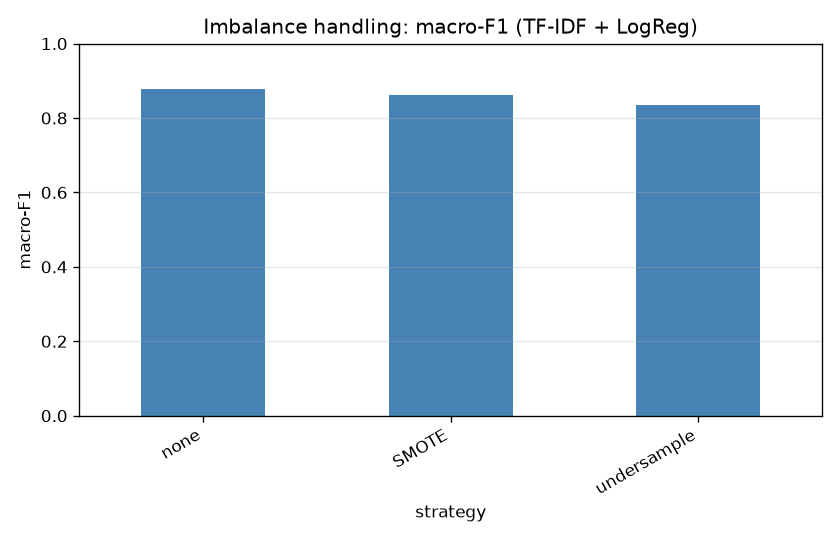
\includegraphics[width=0.55\linewidth]{imbalance_f1.png}
\caption{Macro F1 for each resampling strategy.}
\end{figure}

This is the most striking result of the study. Without any treatment, the baseline
reaches 0.836 accuracy while its neutral recall is exactly zero, which means it never
recognises a neutral review. SMOTE creates synthetic neutral examples by interpolating
between neighbours, and it lifts the neutral recall from zero to 0.189 at almost no
cost in macro F1, because it adds minority points rather than discarding majority
data. Under sampling pushes the neutral recall further, up to 0.472, but it does so by
throwing away majority examples, which lowers the accuracy to 0.601 and the macro F1
to 0.505. The honest conclusion is that resampling trades majority accuracy for real
minority recall. SMOTE offers the best balance here, while under sampling would be
preferable if surfacing neutral reviews were the priority.

% ----------------------------- 8. PCA ----------------------------------
\section{Dimensionality reduction}
The TF\,IDF matrix has about 4\,600 columns, one per vocabulary term. We reduce this
with Truncated SVD, which is the variant of principal component analysis suited to
sparse text, since ordinary PCA would centre the data and make the sparse matrix dense.
We then measure the downstream macro F1 of a Logistic Regression.

\begin{table}[H]
\centering
\begin{tabular}{ccc}
\toprule
\textbf{Components} & \textbf{Explained variance} & \textbf{Macro F1} \\
\midrule
50 & 28.1\,\% & 0.528 \\
100 & 37.0\,\% & 0.536 \\
200 & 48.2\,\% & 0.542 \\
300 & 56.0\,\% & 0.550 \\
4\,630 (full) & 100\,\% & 0.555 \\
\bottomrule
\end{tabular}
\caption{Performance against the number of retained components.}
\end{table}

\begin{figure}[H]
\centering
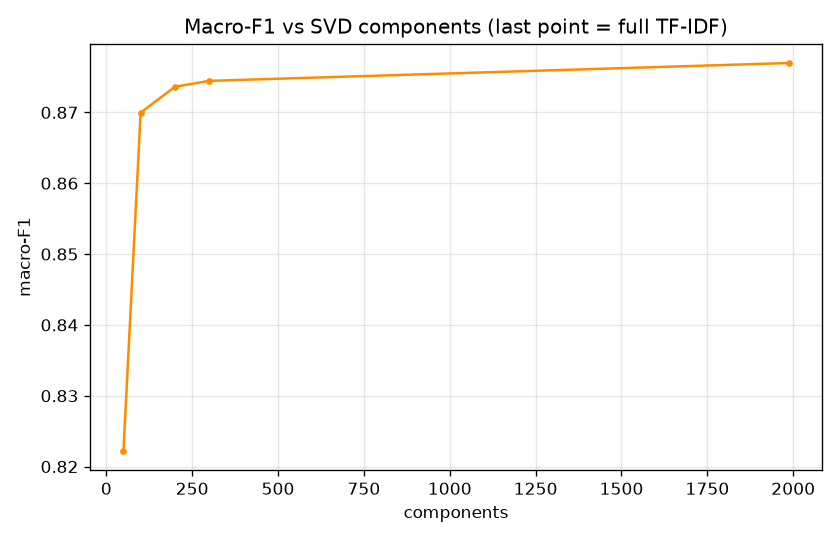
\includegraphics[width=0.6\linewidth]{pca_f1.png}
\caption{Macro F1 as a function of the number of SVD components.}
\end{figure}

Keeping only 300 components, which is about six percent of the features, preserves a
macro F1 of 0.550 against 0.555 for the full representation. Even fifty components
retain 0.528. Dimensionality reduction is therefore an excellent trade off between
speed and accuracy, and it becomes necessary before feeding the otherwise sparse text
to a dense model such as gradient boosting.

% ----------------------------- 9. Pruning ------------------------------
\section{Decision tree pruning}
A single decision tree on TF\,IDF features illustrates pruning very clearly. We follow
the cost complexity path, which gradually removes the least useful branches.

\begin{table}[H]
\centering
\begin{tabular}{cccc}
\toprule
\textbf{ccp\_alpha} & \textbf{Nodes} & \textbf{Train acc.} & \textbf{Test acc.} \\
\midrule
0.0000 (unpruned) & 1\,857 & 0.976 & 0.759 \\
0.0006 & 277 & 0.869 & 0.783 \\
0.0015 & 69 & 0.811 & \textbf{0.786} \\
0.0032 (over pruned) & 29 & 0.779 & 0.770 \\
\bottomrule
\end{tabular}
\caption{Train and test accuracy along the pruning path.}
\end{table}

\begin{figure}[H]
\centering
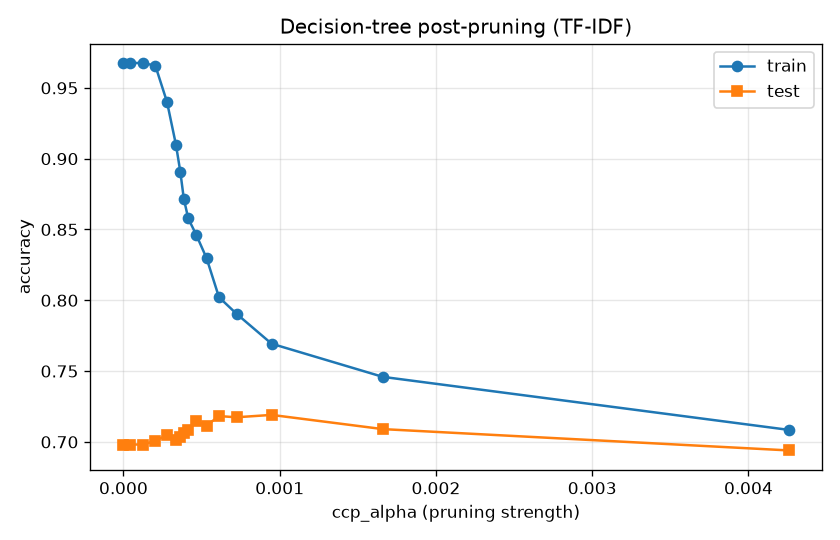
\includegraphics[width=0.6\linewidth]{pruning_accuracy.png}
\caption{Train and test accuracy as the pruning strength increases.}
\end{figure}

The unpruned tree memorises the training set, with 0.976 accuracy in training but only
0.759 in test, a clear sign of over fitting. Pruning reduces the tree from 1\,857
nodes to 69 nodes, raises the test accuracy to 0.786, and shrinks the gap between
training and test from about 0.22 to 0.03. Pruning too aggressively, down to 29 nodes,
starts to under fit. This is the bias variance trade off made visible, and it yields a
tree that is both far smaller and more accurate on unseen data.

% ----------------------------- 10. Early stopping ----------------------
\section{Early stopping}
For the gradient boosting model, which adds trees one at a time, we allow a generous
ceiling of 500 trees and monitor a small validation slice, stopping as soon as the
validation performance stops improving. Training halts after only 88 trees out of 500,
which is roughly six times less computation, with no loss of test quality and a clear
protection against the over fitting that additional trees would bring.

\begin{figure}[H]
\centering
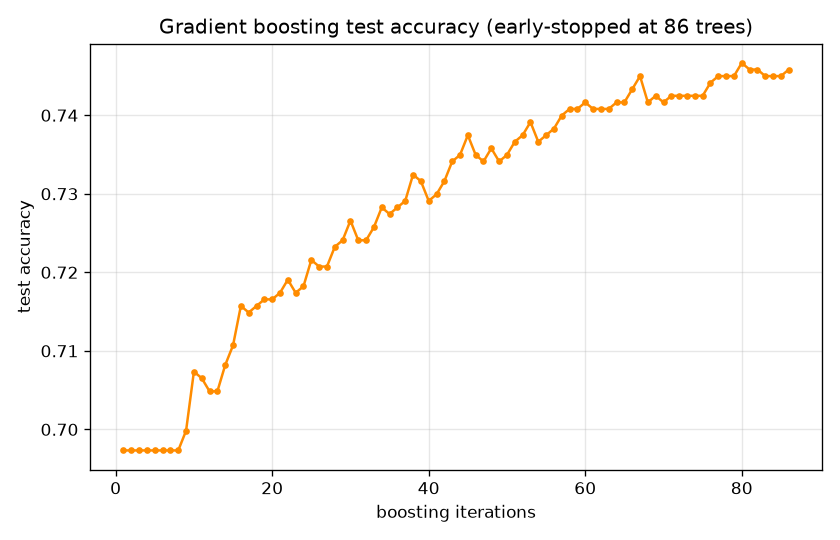
\includegraphics[width=0.6\linewidth]{early_stopping.png}
\caption{Test accuracy as a function of the number of boosting iterations. The model
stops well before the ceiling.}
\end{figure}

% ----------------------------- 11. Discussion --------------------------
\section{Discussion and trade offs}
Taken together, the experiments paint a coherent picture. Simple sparse models win on
short and noisy review text, and TF\,IDF with Naive Bayes is the sweet spot. Accuracy
is the wrong headline metric on this dataset, since a model can reach 0.84 accuracy
while never predicting the neutral class, so the macro F1 and the per class recall are
what we report and discuss. Resampling, and SMOTE in particular, is what allows the
minority class to exist in the predictions, at the cost of some majority accuracy.
Dimensionality reduction buys efficiency for a negligible loss, while pruning and early
stopping both curb over fitting in a measurable way. The embeddings, whether trained
in domain or pre trained on Google News, sit in the middle of the ranking, because
averaging word vectors dilutes the few strong sentiment words that short reviews live
on.

% ----------------------------- 12. Challenges --------------------------
\section{Challenges and future work}
The main difficulties were honest properties of real data rather than bugs. The star
based labels are only a proxy for sentiment, the neutral class is both tiny and
ambiguous, and the text is short, informal and occasionally written in another
language. Heavy de duplication was necessary to avoid leakage between the training and
the test sets, which reduced ten thousand raw rows to 5\,923 usable ones. For future
work we would enable the BERT vectoriser, which is already implemented and runs through
a dedicated script wherever the model hub is reachable, experiment with class weighting
and adjusted decision thresholds as alternatives to resampling, and collect real GitHub
or JIRA issues to complement the app reviews.

% ----------------------------- 13. Conclusion --------------------------
\section{Conclusion}
We delivered a complete and reproducible sentiment pipeline on a real dataset of
Facebook application reviews, compared four vectorisers and five classifiers tuned with
cross validation, and analysed the results with the appropriate metrics. The best model
is TF\,IDF with Naive Bayes at a macro F1 of 0.559. Beyond the numbers, the project
makes a clear methodological point: on an imbalanced problem the accuracy can be
deceptive, the macro F1 tells the truth, and resampling is what gives the minority
class a voice.

\vfill
\begin{center}
\small\textcolor{primary}{Yann MASSOUAM \quad$\cdot$\quad Vénus BAKIKO \quad$\cdot$\quad Faïçal DIELO}
\end{center}

\end{document}
